\chapter{Technical Background}

\section{Topic Material}

\subsection{Formalisations in Computability Theory}

As mentioned before,
this is certainly not the first formalisation of computability theory concepts inside of proof assistants.
Other works however have focused on more traditional models or with certain specific proofs in mind.
These include $\lambda$-calculus in Coq \cite{forster},
partial recursive functions in Lean \cite{carneiro},
and the aforementioned Turing and Abacus machines in Isabelle \cite{urban}.
Other than choices of model and language,
the key difference between those works and this project is the end goal.
The three mentioned above all set about to formalise computability theory from the perspective of their chosen model or models.
This project works with just Cellular Automata and what results can be specifically shown about them.

Additionally the approach in \cite{urban} often involves specifying certain exact indices in lists and having to manipulate these numbers.
This obviously has its technical benefits and is necessary when working with TMs,
but the desire in this work was to take a ``wholemeal'' functional programming approach to the construction where possible.

The existing research that comes closest to both the goals and execution of this project,
is a formalisation of CA in Coq for the purposes of verifying a result about the firing squad problem \cite{firing}.
Their work bases the CA over the naturals $\mathbb{N}$,
and includes an explicit time parameter.
As well as that,
their transition function is based more around individual cells,
and the properties they define are all based around eventually deriving the proof.


\subsection{Cellular Automata}
The concept of CA has been around since the 1940s and were popularised in the 70s with Conway's Game of Life.
However a lot of the names and terminology associated with them comes from Stephen Wolfram \cite{wolfram}.
His work is not entirely formal,
but others have provided their own formalisations of definitions he put forward \cite{yu}.
This was especially useful as an aid in translating the some of the classifications of CA into Isabelle, 
even if their formalisation differed in many other ways.


\section{Technical Material}

\subsection{Cellular Automata}

A Cellular Automaton in general consists of a rectangular grid of cells sitting in some finite dimension,
with each one of these cells in one of a finite number of different states.
Each cell has a neighbourhood
and a rule that determines how a cell changes with each time step,
based off its own state and the states of the cells in its neighbourhood.

All the CA this project is concerned with have cells in one of only two binary states: \mintinline{isabelle}{One} or \mintinline{isabelle}{Zero}.
On diagrams \mintinline{isabelle}{One} is indicated by a filled in black square,
and \mintinline{isabelle}{Zero} by a white square.
In one dimension these are known as \emph{elementary cellular automata}.

This project deals with both one and two dimensional cellular automata.
In the one dimensional case the overall state of the whole automaton can be thought of as a single line of cells,
and in the two dimensional case as cells tiling the plane.
Extensions to higher dimensions are of course possible but not dealt with here.

The neighbourhood used for one dimensional CA here is the simplest possible,
consisting only of a trio of cells including the cell itself in the middle, and the cell to its immediate left and right as seen in \Cref{fig:nbhd_1D}.


\begin{figure}[h]
    \centering
    
\includegraphics[scale=1.7]{neighbourhood_1D.pdf}
    \caption{Neighbourhood of the {\color{blue} blue} cell includes itself and the cells in {\color{red} red}}
    \label{fig:nbhd_1D}
\end{figure}

In two dimensions there are more possible neighbourhoods that still seem natural.
The one used here is known as the \emph{Moore neighbourhood},
made up of the nine cells that form a square including the cell itself as the centre.
Alternatives include the \emph{von Neumann neighbourhood},
which only takes the squares in the cardinal directions from the centre.


\begin{figure}[h]
    \centering
    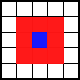
\includegraphics[scale=1.7]{neighbourhood_moore.pdf}
    \caption{Moore neighbourhood}
    \label{fig:moore}
\end{figure}

When showing the development of a one dimensional CA over time,
it is best represented by multiple rows of cells, 
with each new row representing the state at the next time step,
and with time increasing downwards along the y-axis.
It's important to remember that the whole structure depicted never exists at any point in time,
only the one dimensional slices across.

\begin{figure}[h]
    \centering
    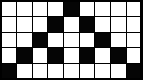
\includegraphics[scale=1.7]{rule26.pdf}
    \caption{Rule 26 traces a Sierpi\'{n}ski triangle over time}
    \label{fig:rule26}
\end{figure}

A two dimensional CA is of course visually shown as a cell diagram in the plane,
with changes over time indicated via multiple diagrams adjacent to each other
and time flowing forward from left to right.

\begin{figure}[h]
    \centering
    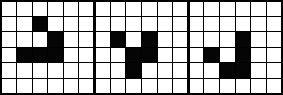
\includegraphics[scale=1.7]{glider.pdf}
    \caption{3 steps of a ``glider'' in Game of Life}
    \label{fig:glider}
\end{figure}

Rules can be specified by a mathematical formulation based on the cells in a neighbourhood as they are in the Game of Life,
or just explicitly defined by listing all inputs and outputs.
For elementary CA the rule is derivable from its Wolfram code which is also used as the name of the rule e.g. Rule 110.
However in this project explicit representations were used.
As an example part of the definition of Rule 110 is given in \Cref{table:rule110}

\begin{table}[htbp]
    \centering
    \begin{tabular}{c|ccc}
        % \hline
        Neighbourhood & $\blacksquare \blacksquare \blacksquare$ & $\blacksquare \blacksquare \square$ & $\blacksquare \square \blacksquare$  \\
         \hline
         Output & $\square$ & $\blacksquare$ & $\blacksquare$
        %  \hline
    \end{tabular}
    \caption{Rule 110}
    \label{table:rule110}
\end{table}


\subsection{Isabelle}

Isabelle as a proof assistant allows us to to define algebraic datatypes and pure total recursive functions,
using pattern matching, guards, and conditionals in a syntax very similar to Haskell's.
Function types are represented in the usual currying friendly way for multiple arguments.
For instance see \Cref{code:example_fun} below.

\begin{myminted}{Functions demonstrating multiple arguments and pattern matching}{example_fun}
    fun get_cell :: "state => int => int => cell" where
    "get_cell s x y = s!(nat x)!(nat y)"

    fun apply_nb :: "(cell => cell) => neighbourhood => neighbourhood" where
    "apply_nb f (Nb a b c) = Nb (f a) (f b) (f c)"
\end{myminted}

On top of these we can state and prove theorems using all the usual first order logic connectives, quantifiers and operators,
along with some Isabelle specifics.
There are multiple different ways of writing proofs in Isabelle,
with some being written in the more human-readable Isar language
and others simply being a chain of commands to apply.
Both kinds will be made use of in the project.

\begin{myminted}{An example statement of theorem named ``t1'' along with proof}{example_thm}
    theorem t1 :"n>0 ==> ca yields State (run ca n)"
      apply(simp add: yields_def)
      apply(rule exI)
      apply(rule conjI)
      apply(auto)
      done
\end{myminted}

Strictly speaking everything in quotation marks is part of HOL,
the logic that Isabelle runs on by default,
and the language most of the actual programming happens in.
However for the sake of simplicity throughout this report the whole language and infrastructure shall simply be referred to as``Isabelle''.
Each file in Isabelle is referred to as a \mintinline{isabelle}{theory},
and is a selection of definitions and proofs.
These theories may draw in and reference other predefined or user made theory files as dependencies, in the same way as any programming language uses libraries.

